\documentclass[conference]{IEEEtran}
\IEEEoverridecommandlockouts
% The preceding line is only needed to identify funding in the first footnote. If that is unneeded, please comment it out.
\usepackage{cite}
\usepackage{amsmath,amssymb,amsfonts}
\usepackage{algorithmic}
\usepackage{graphicx}
\usepackage{textcomp}
\usepackage{xcolor}
\usepackage[spanish]{babel}
\usepackage[utf8]{inputenc}
\usepackage{listings}
\usepackage{color}
\usepackage{caption}
\usepackage{float}

% A few listings color definition
\definecolor{dkgreen}{rgb}{0,0.6,0}
\definecolor{gray}{rgb}{0.5,0.5,0.5}
\definecolor{mauve}{rgb}{0.58,0,0.82}

% listings styles definition
\lstdefinestyle{pythonStyle}
{
	frame=tb,
	language=Python,
	aboveskip=3mm,
	belowskip=3mm,
	showstringspaces=false,
	columns=flexible,
	basicstyle={\small\ttfamily},
	numbers=none,
	numberstyle=\tiny\color{gray},
	keywordstyle=\color{blue},
	commentstyle=\color{dkgreen},
	stringstyle=\color{mauve},
	breaklines=true,
	breakatwhitespace=true,
	tabsize=3
}

\lstdefinestyle{CStyle}
{
	frame=tb,
	language=C,
	aboveskip=3mm,
	belowskip=3mm,
	showstringspaces=false,
	columns=flexible,
	basicstyle={\small\ttfamily},
	numbers=none,
	numberstyle=\tiny\color{gray},
	keywordstyle=\color{blue},
	commentstyle=\color{dkgreen},
	stringstyle=\color{mauve},
	breaklines=true,
	breakatwhitespace=true,
	tabsize=3
}

\renewcommand\spanishtablename{Tabla}

\begin{document}

\title{HMusket: corrector de secuencias mediante el espectro k-mer basado en Hadoop}

\author{\IEEEauthorblockN{Luis Lorenzo Mosquera}
	\textit{GAC (Grupo de Arquitectura de Computadores)}\\
\IEEEauthorblockA{\textit{Dpto. de Ingeniería de Computadores} \\
A Coruña, Spain \\
luis.lorenzom@udc.es}
}

\maketitle

\begin{abstract}
La alta demanda del análisis de datos genéticos durante la última década ha incrementado la necesidad de software que pueda procesar todo este volumen da datos en tiempos razonables.\\
Una de fases requeridas durante estos análisis es la corrección de secuencias, ya que durante la amplificación de las muestras a secuenciar se pueden introducir errores debido a fallos del ADN Polimerasa.\\
A lo largo de este proyecto se presenta HMusket, una herramienta paralela para sistemas de memoria distribuida implementada con Hadoop y siguiendo el modelo MapReduce, que logra reducir los tiempos de corrección de grandes volúmenes de datos, pudiendo procesar datos del orden de varios Terabytes, siento considera este volumen de datos como Big Data. Llegando a incrementar la corrección de secuencias con una aceleración de 20.7 frente a una versión análoga de memoria compartida. Además de la herramienta se presenta un análisis de las distintas soluciones disponibles actualmente. Esta herramienta esta disponible en https://github.com/luislorenzom/hmusket
\end{abstract}

\begin{IEEEkeywords}
Big Data, MapReduce, Hadoop, Corrector de secuencias
\end{IEEEkeywords}

\section{Introducción}
Debido a la aparición de las tecnologías conocidas como \textit{Next Generation Sequence} (NGS)[*] es posible obtener en poco tiempo grandes volúmenes de datos genéticos procedentes de diversos seres vivos (humanos, animales, plantas, etc). Estos vastos conjuntos de datos se utilizan principalmente para el estudio en detalle de dichos seres. 
No obstante el continuo abaratamiento de estas tecnologías acerca a los científicos hacia nuevos objetivos donde tienen más cabida todos estos datos. Además del ya citado estudio de los seres vivos otros grandes propósitos o campos de estudios donde tienen aplicabilidad estos datos dentro del área de las ciencias de la vida (biología, medicina, etc.) son: la predicción de enfermedades, de carácter/predisposición genética, en un estadio temprano para evitar futuras complicaciones en el paciente. \\

La metagenómica[*] es estudio desde el punto de vista genómico de comunidades microbianas. Este amplio campo ha adquirido gran importancia en los últimos años ya que por medio de estos estudios se puede descubrir el fraude o las malas condiciones en la industria alimentaria, determinar las condiciones medioambientales de una zona e incluso detectar ciertas enfermedades por los patógenos registrados en una muestra. Por último, la farmacogenética[*], disciplina que consiste en la interacción de la información genética adquirida durante la fase de secuenciación junto con una base de conocimiento de las áreas de la farmacología y patología, puede predecir qué fármaco es más efectivo para un paciente, incluso dar lugar al diseño de uno nuevo.
\\

No obstante, para llegar a tales fines y obtener unos resultados confiables son necesarios una serie de pasos previos. Además de obtener una muestra de ADN y secuenciarla, es necesario corregir los datos obtenidos tras la secuenciación ya que durante la fase de amplificación, o síntesis de nuevas copias por medio de técnicas PCR[*], es posible que se incorporen errores debido a algún fallo del ADN Polimerasa[*]. Afortunadamente esta clase de fallos siguen un proceso estocástico y pueden ser corregidas en su mayoría a través de diversos algoritmos.
\\

Dada la problemática anteriormente citada sumada a la gran demanda de datos genéticos que se está produciendo a lo largo de la última década, se tiene como consecuencia que las soluciones tradicionales que corrigen estos errores produzcan un cuello de botella en los estudios anteriormente mencionados. Esto es debido a que la mayoría de las herramientas paralelas para la corrección de errores están desarrolladas para sistemas de memoria compartida. Por lo tanto, su escalabilidad esta limitada por una sola máquina con lo que no logran reducir considerablemente los tiempos de preprocesado de los datos.
\\

El propósito de este trabajo es de proveer a los científicos con una herramienta paralela denominada HMusket para sistemas de memoria distribuida[*] que pueda reducir el tiempo de corrección de las secuencias. Para la implementación de dicha herramienta, resulta de interés la aplicabilidad de las tecnologías Big Data las cuales pueden proporcionar los mecanismos adecuados para el procesamiento de grandes conjuntos de datos genéticos. Además de presentar la herramienta, es de interés detallar las tecnologías utilizadas a lo largo del proyecto (sección II), analizar que otras alternativas hay en el mercado para llevar a cabo tal fin ya sean de memoria compartida o distribuida (sección III), comentar el diseño de la herramienta y los entresijos de la implementación (sección IV) y finalizar con un análisis experimental (sección V)  junto con una serie de conclusiones y trabajo futuro (sección VI).\\

\section{Conocimiento previo}

A continuación se describen brevemente las diversas tecnologías utilizadas en este proyecto.

\subsection{MapReduce}
Modelo de programación paralelo propuesto por Google\cite{mapreduce} que surge ante la necesidad de procesar cantidades ingentes de datos de forma distribuida. Este paradigma consta de dos operaciones fundamentales derivadas de la programación funcional: Map y Reduce.\\

La operación Map, convierte un par (clave, valor) en otro conjunto intermedio de datos en el mismo formato de tupla. Dicho formato hace mucho más eficiente el procesado de los datos y una futura reconstrucción de los mismos. Puede verse un ejemplo de esta operación de esta operación en el listing \ref{map}.\\

\begin{lstlisting}[style=pythonStyle, caption=Ejemplo de operación Map, label=map]
# Se inicializa un dataset con unos valores
dataset = [1, 2, 3, 4, 5]
# Se realiza la operacion de elevar al 
# cuadrado, mediante una funcion lambda
# y el resultado se almacena como una lista
dataset = list(map(lambda x: x**2, dataset))
# dataset = [1, 4, 9, 16, 25]
\end{lstlisting}

Por otro lado, la operación Reduce utiliza los conjuntos de datos, ya sean intermedios generados por las operaciones Map, o lo datos originales, para agruparlos y obtener un resultado final (véase listing \ref{reduce} para un ejemplo de código reduce).

\begin{lstlisting}[style=pythonStyle, caption=Ejemplo de operación Reduce, label=reduce]
# Se inicializa un dataset con unos valores
dataset = [1, 2, 3, 4, 5]
# Al igual que en el ejemplo anterior 
# se utiliza una funcion lambda, en este caso
# la multiplicacion de dos numeros
value = reduce((lambda x, y: x * y), dataset)
# value = 120
\end{lstlisting}

\subsection{Apache Hadoop}
Hadoop \cite{hadoop} es un framework de código abierto desarrollado en Java orientado a la ejecución de aplicaciones distribuidas en un entorno cluster y al procesamiento paralelo y eficiente de grandes conjuntos de datos. Hasta la fecha Hadoop es la implementación más utilizada y popular del modelo MapReduce.

\subsection{Hadoop Distributed File System (HDFS)}
HDFS\cite{hadoop_hdfs} es un sistema de ficheros distribuido que permite a las aplicaciones del ecosistema Hadoop trabajar con una alta tolerancia a fallos. Además, facilita el acceso a los datos que se encuentran repartidos entre todo el conjunto de computadores que componen el cluster. Es relevante destacar que este sistema de ficheros no cumple en su totalidad con el estándar POSIX[*] lo cual provoca incompatibilidades con la mayoría del software existente.

\subsection{Hadoop Sequence Parser (HSP)\cite{hsp}}
Uno de los principales inconvenientes que tiene trabajar con Hadoop es la entrada de parámetros tanto en las clases Map como en las Reduce. Por defecto el framework ofrece formatos de entrada para tipos de dato comúnmente usados, como por ejemplo texto, valores numéricos, etc. Esto quiere decir que los formatos que utilizan los formatos Fasta o Fastq\cite{fastq} no pueden ser procesados de una manera directa. Como solución a este problema, no solo para este proyecto sino para otros, se desarrolló una librería para el procesamiento de conjuntos de datos de secuencias Fasta/Fastq que se almacenan en HDFS. De esta manera se evita un preprocesado de los datos al inicio del programa con el consecuente cuello de botella que implica.

\subsection{Java Native Interface (JNI)}
JNI\cite{jni} es una librería que permite que un determinado código Java ejecutado sobre la máquina virtual envíe y reciba llamadas desde código nativo, es decir, programas y/o librerías desarrolladas en C, C++ o Ensamblador.

\section{Trabajos relacionados}

A lo largo de esta sección se presentarán las diferentes soluciones que actualmente hay disponibles para realizar la tarea de corrección de secuencias además de un breve comentario acerca de su funcionalidad y/o limitaciones.

\subsection{Memoria compartida}

Dentro del grupo de soluciones que explotan los sistemas de memoria compartida cabe destacar las soluciones basadas en GPU como son CUDE-EC[*] y DecGPU\cite{decgpu}. Estas herramientas utilizan un algoritmo basado en la realización de lecturas cortas del genoma, lo que no provee una solución completa de errores ni una alta precisión en los resultados (no se da cobertura total a todas las regiones genómicas). No obstante, al estar desarrolladas para GPUs presentan una escalabilidad muy alta debido a la alta capacidad computacinal de estos dispositivos.\\

Otra solución que utiliza un algoritmo basado en lecturas cortas del genoma, pero usando CPU en lugar de GPU, es SOAP Corrector[*]. Recientes versiones de este programa utilizan, en unas determinadas operaciones de su pipeline, un método basado en el grafo De Brujin[*]. Esto permite reducir drásticamente el uso de memoria en casos donde el tamaño del genoma pueda presentar problemas.\\

Siguiendo con las soluciones que están basadas en modelos de grafos se encuentra Reptile[*]. Este software hace uso de un grafo Hamming[*], el cual se combina junto con el análisis del espectro k-mer[*], para resolver las posibles ambigüedades que se encuentren en el genoma o región genómica a corregir, muy útil en casos que presenten errores de translocación. Sin ser un software basado en un modelo de grafos, SGA[*] consigue optimizar el uso de la memoria utilizando la trasformada de Burrows-Wheeler[*] y el FM-Index[*] para representar el espectro k-mer de la región genómica.\\

Además de los métodos de lecturas cortas y de utilización de grafos hay alternativas basadas en modelos probabilísticos como por ejemplo Quake[*]. Este corrector utiliza la probabilidad acumulada[*] de los k-mer que conforman el genoma para poder clasificar si se trata de un error o no.\\

Otros programas combinan soluciones ya mencionadas como pueden ser algoritmos basados grafos y modelos probabilísticos. Un ejemplo es Hammer[*], que se compone de una solución basada en un grafo Hamming y un modelo probabilístico similar al que implementa Quake.\\

Musket\cite{musket}, es un software que permite la corrección de datos genómicos en base al espectro k-mer del mismo. Este programa esta paralelizado mediante la API[*] OpenMP[*] pudiendo acelerar parte de su pipeline de corrección de datos entre los distintos cores de la máquina donde se esta ejecutando. Para realizar dicha aceleración, los desarrolladores decidieron abordar esta problemática utilizando un patrón maestro/esclavo[*], el cual permite minimizar problemas relacionados con el desbalanceo de carga e hilos ociosos. Además de lo ya citado anteriormente, este corrector ofrece gracias al uso del análisis del espectro k-mer una gran cobertura de todo el código genético procesado.\\


Por último, cabe destacar que algunos correctores hacen uso de arrays de sufijos[*], como por ejemplo HiTEC[*], el cual instancia el genoma con distintos k-mers para posteriormente construir esos arrays y analizar los posibles errores. SHREC[*] es otra herramienta que utiliza un método parecido por HiTEC pero para la detección de indels[*] y sustituciones.\\

Según la literatura reciente\cite{comparative}, Musket ha demostrado ser la herramienta que mejores resultados proporciona en relación a la corrección de código y la cobertura del mismo, obteniendo un Valor-F[*] del 81\% corrigiendo un dataset de cobertura media, mientras que el resto de herramientas fallaban en medio del proceso o no alcanzaban la misma precisión.

\subsection{Memoria distribuida}
Dada la reciente necesidad de un post-procesado masivo de datos apenas hay soluciones de memoria distribuida para la corrección de errores. Solo destacan dos soluciones en este paradigma:\\

Quake es una adaptación de la versión de memoria compartida al entorno Hadoop, donde se distribuye el conjunto de datos de secuencias entre varios nodos y se ejecutan varias instancias del citado software. Sin embargo, esta versión ha sido descartada por sus propios desarrolladores ya que obtiene tiempos superiores a la versión de memoria compartida.\\

CloudRS\cite{cloudrs}, es otra herramienta implementada para el entorno Hadoop mediante el paradigma MapReduce. Pese a ser una solución de memoria distribuida no proporciona unos resultados con gran cobertura genética. Además, requiere un preprocesado del conjunto de secuencias de entrada antes de copiarlo a HDFS, lo cual causa un cuello de botella de considerables dimensiones por el intenso tráfico de E/S a disco. Hmusket consigue eliminar dicho preprocesado gracias al uso de la librería HSP como se ha mencionado en la sección II-D\\

\section{Diseño e implementación}

En líneas generales la motivación de este proyecto es distribuir entre varios nodos un determinado conjunto de datos genéticos ya sea Fasta o Fastq en modo single-end[*] o paired-end[*] y ejecutar varias instancias de Musket de forma simultánea. Finalmente se debe realizar una operación merge de todas las salidas obtenidas en el cluster.\\
El principal motivo para utilizar Musket como corrector subyacente en lugar de otros similares (e.g. Reptile) es porque, como ya se citó anteriormente, la literatura reciente demuestra que este es el corrector con mayor precisión hasta la fecha.\\

Para el desarrollo del presente trabajo se tuvieron que completar dos hitos que componen la totalidad del proyecto. En posteriores párrafos se detallan en profundidad, pero en esencia dichos objetivos fueron la creación de una librería para ejecutar el algoritmo de Musket, y la creación de una aplicación distribuida mediante Hadoop denominada HMusket. Pudiendo de esta manera dividir los conjuntos de datos de entrada entre los distintos nodos de computo y que posteriormente ejecutar la librería que contiene el algoritmo de corrección de secuencias.\\

No obstante antes de detallar el diseño e implementación de HMusket conviene dar una visión general de como están estructuradas las aplicaciones Hadoop.

\subsection{Estructura general de una aplicación Hadoop}
Las aplicaciones Hadoop, por lo general, consiste en: un programa driver donde se configura la aplicación: ficheros de entrada, salida, formatos con los que va a trabajar, etc. A su vez, en el driver se crea el Job a ejecutar en el clúster, al cual se le indican con que clases Map y Reduce debe trabajar y el orden de las mismas.\\
La implementación de dichas clases Map y Reduce siguen el siguiente ciclo de vida o flujo:

\begin{itemize}
	\item Setup: operación que se realiza al inicio de la etapa Map o Reduce
	\item Map o Reduce: operación/función que se realiza por cada par (clave, valor) del conjunto de datos a manejar.
	\item Cleanup: operación que se realiza al final de la etapa Map o Reduce.
\end{itemize}

\subsection{Desarrollo de HMusket}
HMusket sigue la estructura indicada en el aparatado anterior. En el driver se recogen los parámetros de entrada que se reciben al lanzar la aplicación (e.g. ruta al fichero de entrada Fasta/Fastq). Posteriormente, se invoca al método parse de la clase CLIParse (véase figura \ref{class_diagram}) el cual evalúa la obligatoriedad de dichos parámetros, configura parte del driver y genera una cadena que conforma los argumentos que recibirá la librería de Musket para ejecutar el algoritmo de corrección de secuencias.\\
Una vez configurado el driver, se establecen los ficheros de entrada y salida de los mappers: tanto el que procesa los dataset single-end como el de los pair-end, dependiendo del caso. Para ello se hace uso de las clases InputFormat[*] que proporciona la librería HSP. Esto es necesario para que Hadoop sepa que tipo de información está procesando cada mapper. Es decir, establecer si las secuencias de entrada que esta recibiendo son de tipo Fasta, donde se procesa una cadena para la secuencia bases y otra para el identificador, o Fastq, que a mayores de la cadena de ADN y el identificador, proporciona la opción de añadir un comentario y una segunda cadena que informa de la calidad de las bases. De esta manera cada mapper recibe un parte proporcional del dataset, evitando así que, por ejemplo, un mapper reciba de entrada secuencias o cadenas de calidad desparejadas, cualquier tipo de pre-procesado del dataset y cuellos de botella. El único requerimiento para que este método funcione es subir previamente el dataset a HDFS algo inherente al uso de cualquier aplicación Hadoop.\\

Los distintos mappers que se manejan en HMusket instancian durante la fase setup un PrintWriter[*] para cada dataset que manejan (si es modo single-end solo trabaja con uno, mientras que el mapper de los datasets en formato pair-end utiliza dos). Posteriormente, en la etapa map, se escribe toda la información de entrada al disco duro local del nodo de cómputo. Esto es necesario porque la librería que ejecuta Musket utiliza I/O mediante sistemas de ficheros basados es POSIX, mientras que para poder distribuir y poder trabajar adecuadamente con Hadoop se tiene que utilizar el sistema de ficheros distribuidos HDFS.\\
Finalmente en la etapa cleanup se cierra el buffer de escritura del/o los PrintWriter y se efectúa la llamada al código nativo de Musket, pasándole por parámetro el string que conforma los argumentos necesarios, generado previamente en la clase CLIParse. Tras la ejecución nativa de Musket, se eliminan los archivos locales que se utilizaron para la entrada de Musket y se copian las salidas a HDFS. Finalmente se hace un merge de todas las salida de cada mapper para obtener un único fichero de salida.\\

La nula referencia a las clases reduce, tal y como se puede apreciar en la figura \ref{class_diagram} y en los párrafos superiores, es debido a que para el diseño de HMusket no es considero necesario una etapa reduce, ya que solo interesa dividir el conjunto de datos y aplicar la función corregir de Musket.

\begin{lstlisting}[style=CStyle, caption=Cabecera JNI generada]
/*
 * Class:     es_udc_gac_hmusket_MusketCaller
 * Method:    callMusket
 * Signature: (Ljava/lang/String;)V
 */
JNIEXPORT void JNICALL Java_es_udc_gac_hmusket_MusketCaller_callMusket (JNIEnv *, jobject, jstring);
\end{lstlisting}

\begin{figure*}
	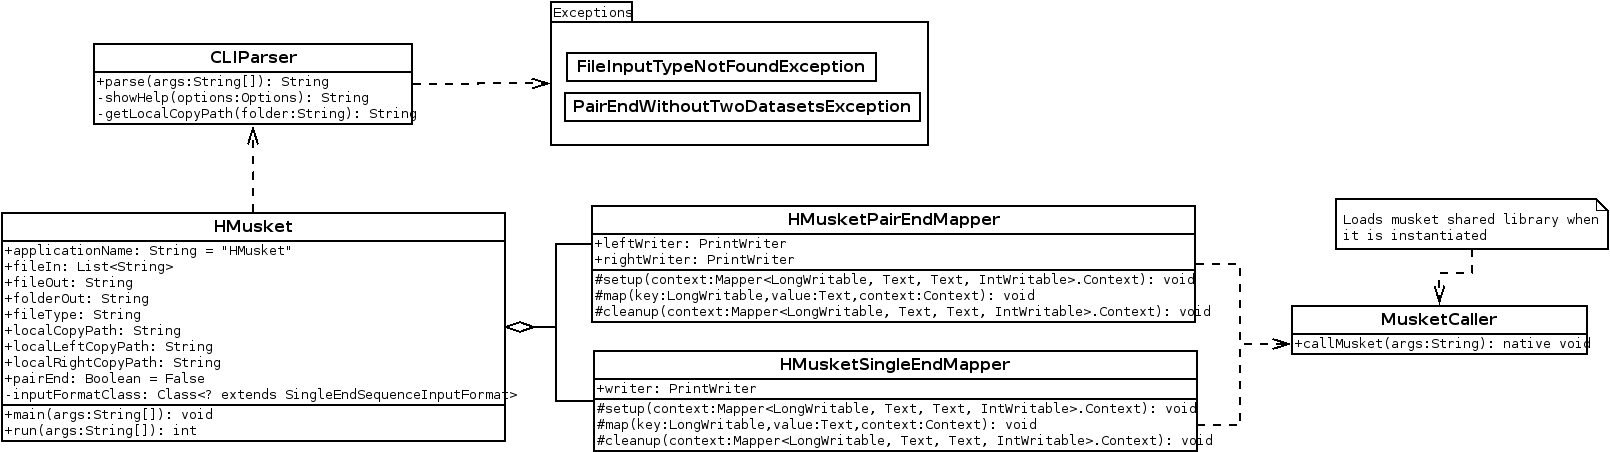
\includegraphics[width=\textwidth]{figures/hmusket.png}
	\caption{Diagrama de clases de HMusket}
	\label{class_diagram}
\end{figure*}

\subsection{Creación e integración de la librería}
Para poder realizar la llamada a código nativo es necesario convertir el software Musket en una librería compartida[*]. Posteriormente esa librería debe set instalarla en el cluster Hadoop para que cualquier aplicación del ecosistema pueda hacer uso de la misma.\\
Para efectuar esta tarea hay que crear una clase dentro del proyecto Java, en este caso fue la clase MusketCaller, donde se especifique que durante la fase de instanciación cargue la librería nativa. Además de esta indicación se tiene que crear un método con la etiqueta ``native'', al igual que en los métodos abstractos tan solo se debe especificar la firma.\\
A continuación utilizando el comando ``javac'' se compila dicha clase generando un fichero .class, este fichero es requerido para generar el fichero de cabeceras (.h), por medio del comando ``javah'' para posteriormente darle una implementación.\\
Dicha implementación debe ser incluida en un fichero C o C++ donde implemente la firma indicada en el fichero de cabeceras y por último realizar la llamada a la aplicación Musket.\\
Para poder realizar esta llamada como si fuera una librería en vez de un binario, se requiere una única modificación en el makefile de Musket para añadir a los flags del compilador necesarios para crear una librería compartida (``-fPIC'' y ``-shared''). Una vez compilada se añade al directorio \$HADOOP\_HOME/lib/native y por último se declarara la función main, del proyecto Musket, dentro del código C desarrollado.

\section{Evaluación experimental}
En primer lugar se detallará el entorno, tanto software como hardware, donde se realización las pruebas para maximizar la reproducibilidad de los experimentos que se muestran a lo largo de esta sección. Posteriormente se indicara el estudio realizado sobre Musket para conocer la horquilla de tiempos a mejorar y los posibles cuellos de botella.\\
Para concluir, se expondrán los experimentos, resultados y conclusiones acerca de HMusket.

\subsection{Entorno de pruebas}
Para la realización de las diversas pruebas expuestas a lo largo de los siguientes párrafos se utilizó la cabina 0 del cluster Plutón del Departamento de Ingeniería de Computadores, el cual consta con 18 nodos de cómputo con características se muestran en la tabla \ref{node_especification}:\\ 

\begin{table}[t]
	\begin{center}
		\begin{tabular}{|l|l|}
			\hline
			\textbf{Modelo CPU} & 2 × Intel Xeon E5-2660 Sandy Bridge-EP \\ \hline
			\textbf{Velocidad/Turbo CPU} & 2.20 GHz/3 GHz \\ \hline
			\textbf{Cores por CPU} & 8 \\ \hline
			\textbf{Threads por core} & 2 \\ \hline
			\textbf{Cores/Threads por nodo} & 16/32 \\ \hline
			\textbf{Cache L1/L2/L3} & 32 KB/256 KB/20 MB \\ \hline
			\textbf{Memoria RAM} & 64 GB DDR3 1600 Mhz \\ \hline
			\textbf{Discos} & 1 × HDD 1 TB SATA3 7.2K \\ \hline
			\textbf{Redes} & InfiniBand FDR y Gigabit Ethernet \\ \hline
		\end{tabular}
		\caption{Especificaciones de un nodo de computo}
		\label{node_especification}
	\end{center}
\end{table}

En resumen, el cluster cuenta con 1 nodo de login y 18 nodos de cómputo con un total de 288 cores físicos (576 threads) y 1.152 TB de memoria. El sistema operativo que se ejecuta en estos servidores es Rocks 6.1[*] una distribución para entornos cluster basada en CentOS[*] 6.9, mientras que el kernel utilizado es 2.6.32.x. La maquina virtual de java utlizada ha sido OracleJDK 1.7.0\_80. Por último Musket ha sido compilado usando la suite de GNU en su versión 6.3.1.\\

Para la realización de pruebas en el cluster se utilizo la versión 3.1 de BDEv[*], por medio de esta herramienta se puede desplegar un cluster Hadoop con todo su ecosistema de aplicaciones, pudiéndolo configurar de manera sencilla, simplemente hace falta tener una versión del JRE[*] en el entorno. Además de todo esto, BDEv provee de estadísticas e informes de evaluación acerca de como fue el rendimiento de la aplicación durante la ejecución. No obstante, el principal motivo para utilizar esta herramienta fue para poder ejecutar la aplicación distribuida en el sistema de colas del cluster, ya que de por si solo, el cluster no cuenta con el entorno Hadoop para los usuarios y actualmente no hay una solución unificada para la integración este tipo de frameworks en los sistemas de colas.\\

Durante el análisis de Musket y HMusket se utilizaron dos dataset, uno con formato single-end de 49995929 secuencias de tamaño 100, y otro con formato pair-end (es decir, dos ficheros) de 69247248 secuencias (cada uno) de tamaño 101 cada una, ambos de tipo Fastq y todo esto generando un espectro para k-mers de tamaño 2.\\

\subsection{Análisis Musket}
Dado que Musket es un software acelerado mediante OpenMP (memoria compartida) el número máximo de threads con los que se pudo evaluar en el cluster fueron 16, y teniendo en cuenta que se requieren por lo menos 2 threads para funcionar (debido a patrón maestro/esclavo) se decidió evaluar el rendimiento de la aplicación con hilos de 2 a 16 en potencias de 2, es decir: 2, 4, 8, 16.\\

Tal y como se puede apreciar en la tabla \ref{musket_experiment_result} la paralelización de Musket presenta un carácter lineal pudiendo alcanzar una aceleración de aproximadamente 4.6 para el dataset single-end y 8.6 para el dataset pair-end. Resulta curioso, que siendo el dataset pair-end el doble de grande lo procese a en menos tiempo, esto puede ser debido a los k-mers que conforman el espectro del segundo dataset (pair-end) son menores y por lo tanto se repiten más que en el primer dataset, por tanto la evaluación de los mismos se efectúa de una manera más rápida. Respecto a las aceleraciones obtenidas en el proceso experimental, se puede concluir que Musket escala al aumentar el número de cores.

\begin{table}[t]
	\centering
	\begin{tabular}{|l|l|p{1.5cm}|p{1.3cm}|l|}
		\hline
		\textbf{Dataset} 	& \textbf{Threads} 	& \textbf{Número de secuencias} & \textbf{Tamaño secuencias} & \textbf{Tiempo}	\\ \hline
		Single-end 	& 2			& 49995929           & 100           & 13h: 29min: 21sec 	\\ \hline
		Single-end 	& 4			& 49995929           & 100           & 08h: 44min: 17sec	\\ \hline
		Single-end 	& 8			& 49995929           & 100           & 04h: 44min: 12sec 	\\ \hline
		Single-end 	& 16		& 49995929           & 100           & 02h: 52min: 17sec 	\\ \hline \hline
		Pair-end 	& 2			& 69247248           & 101           & 13h: 30min: 02sec 	\\ \hline
		Pair-end 	& 4			& 69247248           & 101           & 04h: 30min: 15sec	\\ \hline
		Pair-end 	& 8			& 69247248           & 101           & 02h: 24min: 34sec 	\\ \hline
		Pair-end 	& 16		& 69247248           & 101           & 01h: 33min: 41sec 	\\ \hline
	\end{tabular}
	\caption{Tabla experimental de Musket}
	\label{musket_experiment_result}
\end{table}

\begin{table*}[]
	\begin{tabular}{|p{1.3cm}|p{1cm}|l|l|l|p{1.5cm}|p{1.3cm}|p{2.2cm}|p{2.2cm}|}
		\hline
		\textbf{Dataset} &	\textbf{Número de nodos} & \textbf{Mapper/Nodo} & \textbf{Threads/Nodo} & \textbf{Memoria/Mapper} & \textbf{Número de secuencias} & \textbf{Tamaño secuencias} & \textbf{Tiempo} & \textbf{Tiempo del merge}	\\ \hline
		Single-end &	4 & 1 & 16 & 50 GB & 49995929 & 100 & 0 h: 25 min: 34 seg	& 2 min: 05.514 seg	\\ \hline
		Single-end &	4 & 2 & 8 & 25 GB & 49995929 & 100 & 0 h: 09 min: 50 seg	& 1 min: 22.847 seg	\\ \hline
		Single-end &	8 & 1 & 16 & 50 GB & 49995929 & 100 & 0 h: 13 min: 39 seg	& 2 min: 07.445 seg	\\ \hline
		Single-end &	8 & 2 & 8 & 25 GB & 49995929 & 100 & 0 h: 08 min: 18 seg	& 1 min: 34.217 seg	\\ \hline \hline
		Pair-end &	4 & 1 & 16 & 50 GB & 69247248 & 101 & 0 h: 42 min: 06 seg	& 5 min: 22.472 seg	\\ \hline
		Pair-end &	4 & 2 & 8 & 25 GB & 69247248 & 101 & 0 h: 30 min: 50 seg	& 6 min : 22.166 seg	\\ \hline
		Pair-end &	8 & 1 & 16 & 50 GB & 69247248 & 101 & 0 h: 23 min: 37 seg	& 5 min: 18.541 seg	\\ \hline
		Pair-end &	8 & 2 & 8 & 25 GB & 69247248 & 101 & 0h: 16 min: 22 seg	& 5 min: 25.067 seg \\ \hline
	\end{tabular}
	\caption{Tabla experimental de HMusket}
	\label{hmusket_experiment_result}
\end{table*}

\subsection{Análisis HMusket}
Para realizar las pruebas de HMusket se estudiaron y valoraron las posibles combinaciones de mapper por nodos que podían ser más eficientes a la hora de efectuar las funciones. Debido a que cada nodo se compone de 2 procesadores de 8 núcleos cada uno, se estableció como máxima repartir en cada nodo a lo sumo 1 mapper por cada procesador, es decir, 1 o 2 mappers por cada nodo de computo. Esto implico, que se tenga que ajustar la memoria y el heap de los mappers (50Gb en caso de 1 mapper y 25Gb en caso de 2 mappers por nodo y en ambos casos se establece el 80\% de la memoria para el heap) por lo tanto, las combinaciones que se decidieron realizar para el experimento son los que se muestran en la tabla \ref{hmusket_experiment_result} junto con los resultados obtenidos en las diferentes pruebas.\\

Durante la realización de los experimentos se tuvieron que efectuar 5 ensayos distintos para cada prueba. El motivo de esto fue evitar la obtención de datos inexactos. Ya que como se mencionó en apartados anteriores, Hadoop es un framework desarrollado en java, y como todo software implementado con esta tecnología el acceso a los recursos proporcionados por la máquina virtual puede introducir ruido en la toma de tiempos (e.g. retardos en el acceso a discos u reserva de memoria). Para la elección del tiempo a introducir en este articulo se realizó una mediana de los 5 valores obtenidos. Se procedió de igual manera para la obtención de los tiempos para realizar la unión de todos los ficheros de salida.\\

Dados los resultados obtenidos en los experimentos realizados con HMusket se puede concluir que el procesamiento que realiza esta herramienta sobre los conjuntos de datos de entrada escala de una manera linear. Obteniendo una aceleración de 20.7 en el procesamiento de los datos en formato single-end. A su vez, para la corrección de los datos en formato pair-end se obtiene un speed-up de 5.7. En ambos casos se utiliza la configuración de 8 nodos ejecutando 2 mapper cada nodo, teniendo que de esta manera dividir la memoria asignada al computador entre 2, recordemos que cada nodo de computo dispone 60 Gb de memoria RAM, de la cual en esta configuración se asignan 25 Gb a cada nodo. Resulta interesante destacar las diferencias entre el uso 2 nodos frente a 1 nodo, justificando de esta manera que el uso de dos nodos por mappers es la configuración óptima. Por ejemplo, en el experimento donde se procesa el conjunto de datos en formato single-end con 4 nodos. En el caso de procesar esta información con 1 solo mapper por nodo se obtienen 25 minutos con 34 segundos. Por contra si se procesa esta información con 2 mappers por nodo se logra reducir este tiempo a  9 minutos y 50 segundos. Es decir, con este cambio de configuración se obtienen una aceleración de 2.6.\\

Respecto a los tiempos obtenidos en la fase del merge de las salidas, se puede apreciar que apenas hay una gran variabilidad entre las distintas configuraciones. No obstante cabe destacar, como es lógico, que a mayor número de mappers se incrementa el tiempo de merge. Pese a esto, hay que recordar que hablamos de conjuntos de datos del orden de 16 Gb (en el caso del single-end) y 44 Gb (22 Gb cada fichero en el caso del modo pair-end) y penalización es del orden de medio minuto.

\section{Conclusiones y trabajo futuro}
Teniendo en cuenta todo lo indicando a lo largo de este artículo se puede concluir con que Musket es una herramienta bastante potente, de hecho de las mejores que hay actualmente, pero nos es capaz de hacer frente a la alta demanda de datos que ha surgido a lo largo de los últimos años.\\
Una buena alternativa para este problema es implementar o reutilizar ese software en un entorno de memoria distribuida, como por ejemplo Hadoop, mediante el paradigma MapReduce, tal y como hace HMusket. De esta manera se pueden evitar cuellos de botella y preprocesados de datos al inicio del análisis, obteniendo aceleraciones de hasta 20.7 además de lograr una escalabilidad lineal en base al número de nodos y mappers utilizados. Cabe destacar que el uso de dos mappers por nodo, en las condiciones experimentales ya indicadas en la tabla \ref{node_especification}, implica una aceleración de hasta 2.6 pese a penalizar esta mejora a la fase de unión de todos los archivos de salida con aproximadamente 30 segundos más.\\ 

Como trabajo futuro sería interesante realizar ciertas modificaciones tanto la librería Musket como en la aplicación Hadoop para evitar las comunicaciones usando la entrada y salida estándar en lugar de ficheros y comparar el rendimiento de esta segunda versión frente a la aquí expuesta. Además, otro estudio que podría ser de gran interés sería analizar como escala el tiempo de merge a medida que aumenta el tamaño del conjunto de datos de entrada y por consiguiente el número de mappers que utiliza la aplicación.\\

% ~~~~~~~~~~~~~~~~~~~~~~~~~~~~~~~~~~~
% Referencias bibliográficas
% ~~~~~~~~~~~~~~~~~~~~~~~~~~~~~~~~~~~

\bibliographystyle{IEEEtran}
\bibliography{IEEEfull}
% ~~~~~~~~~~~~~~~~~~~~~~~~~~~~~~~~~~~
\end{document}
